\section{ILUC Recognition} \label{sec:iluc_recognition}
This section describes a novel algorithm that allows the LUA software to recognize the ILUC. The algorithm combines the lines and edges coming from the profile analysers to form a 3-dimensional representation of the ILUC, similar to how the pipes are already found. The goal of the algorithm is to find the ILUC's direction, radius and centre. For convenience, these values together are termed the \textit{ILUC face}.

The motivation to recognise the ILUC face lies in the ability to perform an accurate pre-line up of the new joint and main line. The new joint's position and orientation can be preemptively adjusted to the ILUC face during line up (see \ref{fig:oop_ILUC_ribs}). This ultimately leads to a more accurate and efficient line up of the new joint and main line, since the ILUC is always centered and fixed in the main line.

The ILUC consists of ten ribs (see \cref{fig:iluc,fig:oop_lua}), each of which is recognised by the profile analysers as a line segment of a specific length ($\sim 1$ cm). In turn, each of these line segments generates two edge points. Consequently, all five profile analysers together can generate up to
\begin{align*}
           & 5 \text{ profile analyser threads}         \\
    \times & 10 \text{ ILUC ribs per profile analyser}  \\
    \times & 2 \text{ ILUC rib edge point per ILUC rib} \\
    =      & 100 \text{ ILUC rib edge points}.
\end{align*}
These edge points are used in algorithm \ref{alg:iluc_recognition} to obtain an estimate of the ILUC face.
\begin{algorithm}
    \begin{algorithmic}[1]
        \State \textbf{function: } \lstinline[language=C]|multiSensorAnalyser_c::checkForILUCFace|
        \State Obtain ILUC rib edge points from the profile analysers
        \State \textbf{If} there are more than six edge points \textbf{then}
        \State \quad Run \lstinline[language=C]|multiSensorAnalyser_c::analyseILUCRibs| (see algorithm \ref{alg:iluc_estimation})
        \State \quad Store the ILUC face
        \State \quad \textbf{If} an ILUC face is found \textbf{then}
        \State \quad \quad Run \lstinline[language=C]|multiSensorAnalyser_c::fitILUCCylinder| (see algorithm \ref{alg:iluc_optimisation})
        \State \quad \quad \textbf{If} the optimised ILUC face has a lower error \textbf{then}
        \State \quad \quad \quad Overwrite the estimated ILUC face with the optimised ILUC face
        \State \quad \quad \textbf{end if}
        \State \quad \textbf{end if}
        \State \textbf{end if}
        \State \textbf{output: } ILUC face
    \end{algorithmic}
    \caption{Pseudo code for ILUC recognition.}
    \label{alg:iluc_recognition}
\end{algorithm}


\subsection{ILUC direction estimation}
The problem of estimating the ILUC face can be solved by combininh circle fits on the ILUC rib edges. The midpoints of these ILUC rib edge circle fits can be used to estimate the ILUC direction. The algorithm is described in algorithm \ref{alg:iluc_estimation}.
\begin{algorithm}[H]
    \begin{algorithmic}[1]
        \State \textbf{function} \lstinline[language=C]|multiSensorAnalyser_c::analyseILUCRibs|
        \State \textbf{input} ILUC rib edge points per profile analyser
        \State Naively group ILUC rib edge points into ILUC rib edges
        \State Fit circles to the ILUC rib edges, yielding ILUC rib midpoints
        \State Remove outliers from the set of ILUC rib midpoints
        \State Get an approximate ILUC direction by fitting a line through ILUC rib edge midpoints
        \State \textbf{If} an approximate ILUC direction is found \textbf{then}
        \State \quad Use approximate ILUC direction to correctly match ILUC rib edge points into edges
        \State \quad Fit circles to the ILUC rib edges, yielding ILUC rib midpoints
        \State \quad Remove outliers from the set of ILUC rib midpoints
        \State \quad Get a corrected ILUC direction by fitting a line through ILUC rib edge midpoints
        \State \quad Use corrected ILUC direction to perform a final circle fit, yielding the ILUC centre and radius
        \State \textbf{end if}
        \State \textbf{output: } ILUC face
    \end{algorithmic}
    \caption{Pseudo code for ILUC face estimation.}
    \label{alg:iluc_estimation}
\end{algorithm}
In line 3 of algorithm \ref{alg:iluc_estimation} the ILUC rib edge points are grouped into ILUC rib edges based on their index in each of the profile analyser threads. This approach is naive, because it does not consider the possibility of a missing edge point. Missing edge points can occur due to a profile analyser not detecting an ILUC rib edge. There are multiple reasons a profile analyser might miss an edge, which are left out of the scope of this discussion. 

Mismatched ILUC rib edges result in slanted circles. This is shown in figure 
\ref{fig:iluc_mismatched_edges}.
\begin{figure}[H]
    \centering
    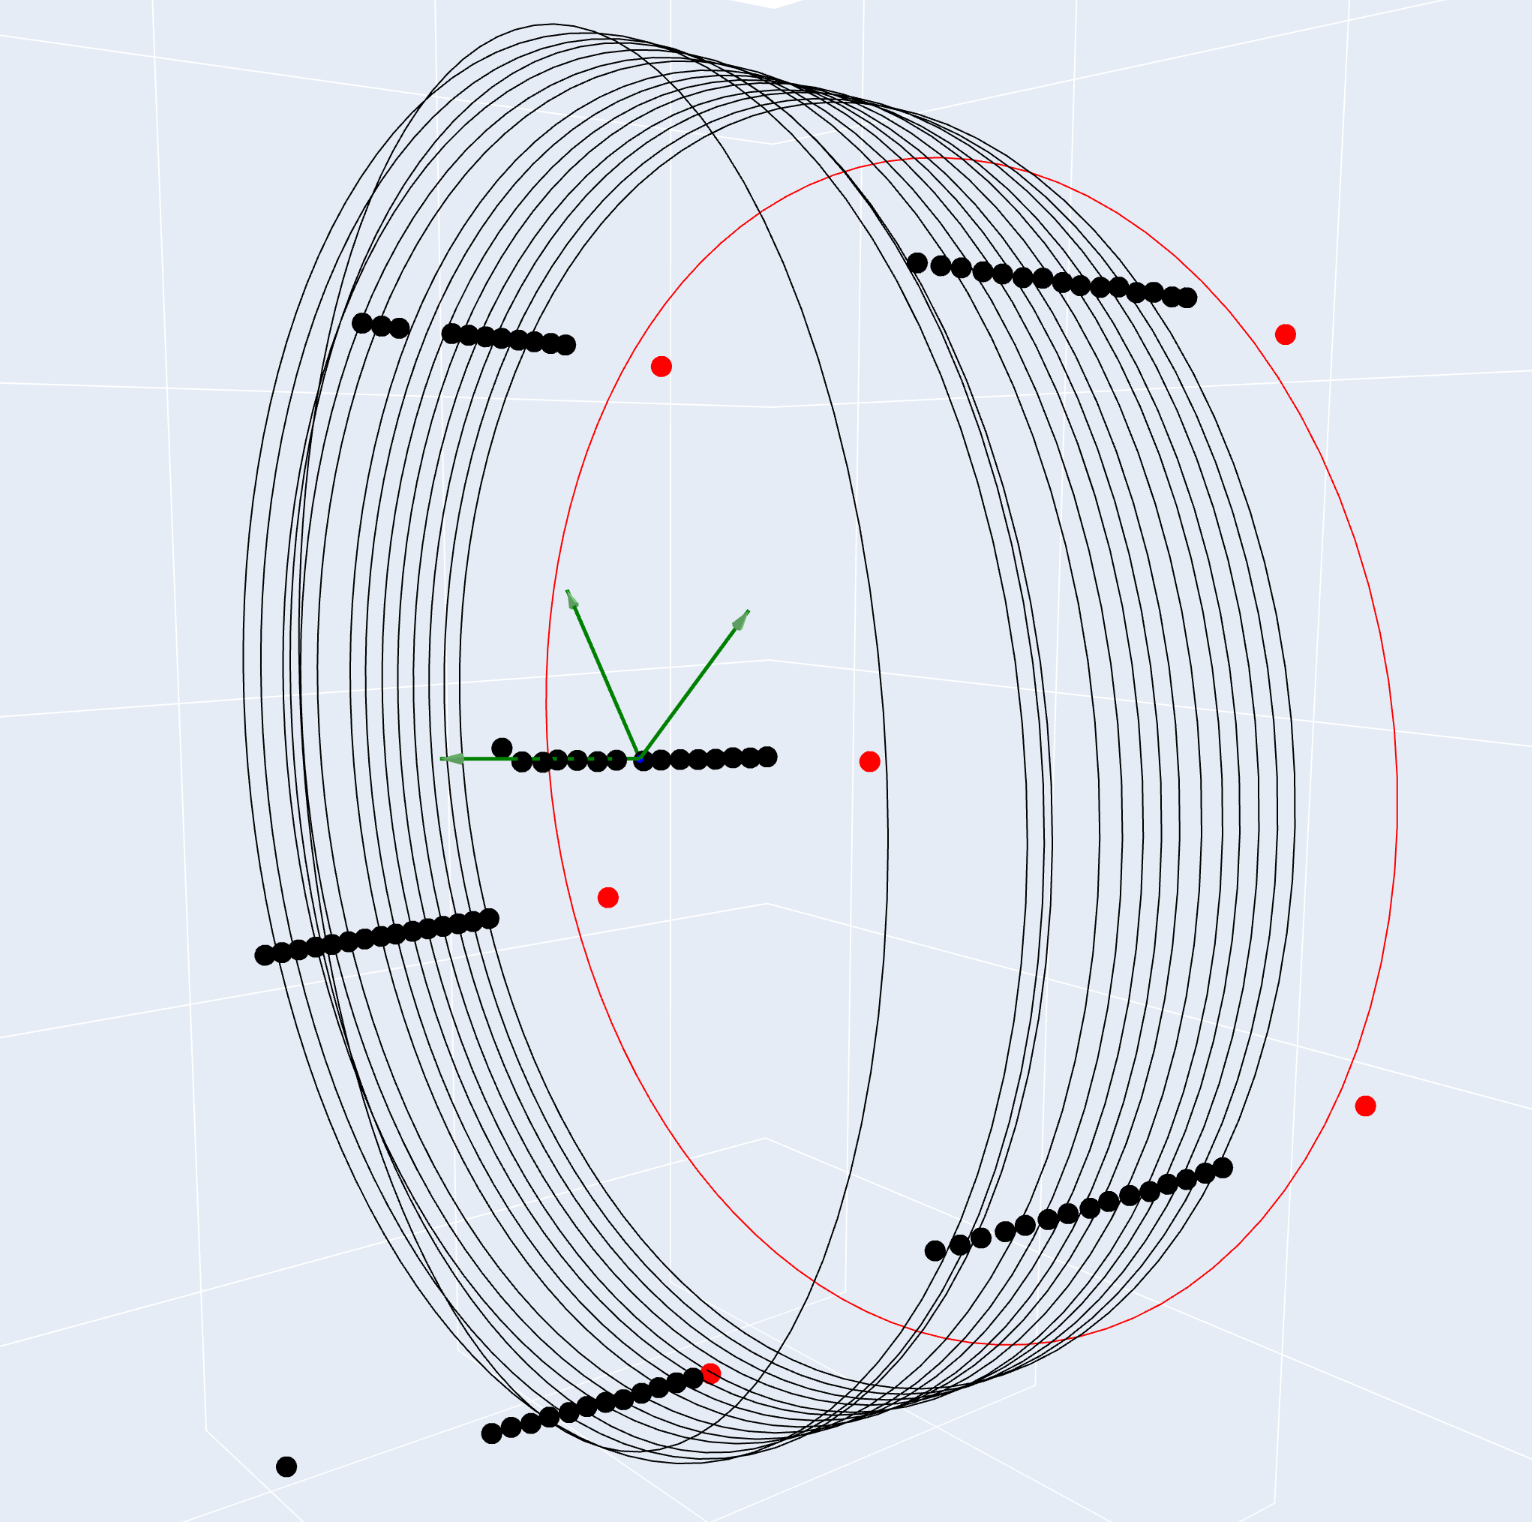
\includegraphics[width=0.8\textwidth]{images/ILUC_naive_grouping.png}
    \caption{Output of algorithm \ref{alg:iluc_estimation}, line 3. Mismatched ILUC rib edges result in slanted circles.}
    \label{fig:iluc_mismatched_edges}
\end{figure}

The midpoints resulting from the possibly mismatched set of ILUC rib edge points are used to obtain a first estimate of the ILUC direction. This estimate is then used to correctly match the ILUC rib edge points into edges. The corrected ILUC direction is then used to perform a final circle fit, yielding the ILUC centre and radius. The ILUC face is then stored and outputted.

\subsection{ILUC direction optimisation}
\begin{algorithm}[H]
    \begin{algorithmic}[1]
        \State \textbf{function} \lstinline[language=C]|multiSensorAnalyser_c::fitILUCCylinder|
        \State \textbf{input} ILUC rib edge points
        \State \dots
        \State \textbf{output: } ILUC face
    \end{algorithmic}
    \caption{Pseudo code for ILUC face optimisation.}
    \label{alg:iluc_optimisation}
\end{algorithm}